% coding:utf-8

%----------------------------------------
%FOSAMATH, a LaTeX-Code for a mathematical summary for basic analysis
%Copyright (C) 2013, Daniel Winz, Ervin Mazlagic, Adrian Imboden, Philipp Langer

%This program is free software; you can redistribute it and/or
%modify it under the terms of the GNU General Public License
%as published by the Free Software Foundation; either version 2
%of the License, or (at your option) any later version.

%This program is distributed in the hope that it will be useful,
%but WITHOUT ANY WARRANTY; without even the implied warranty of
%MERCHANTABILITY or FITNESS FOR A PARTICULAR PURPOSE.  See the
%GNU General Public License for more details.
%----------------------------------------

% coding:utf-8
\section{Darstellung von Funktionen}
\subsection{Polares Koordinatensystem}
Eine Funktion kann auch im Polaren Koordinatensystem definiert werden. 
Dabei wird jeder Punkt durch den Abstand zur Ordinate und den Winkel zur 
x-Achse definiert. 

\begin{figure}[h!]
\centering
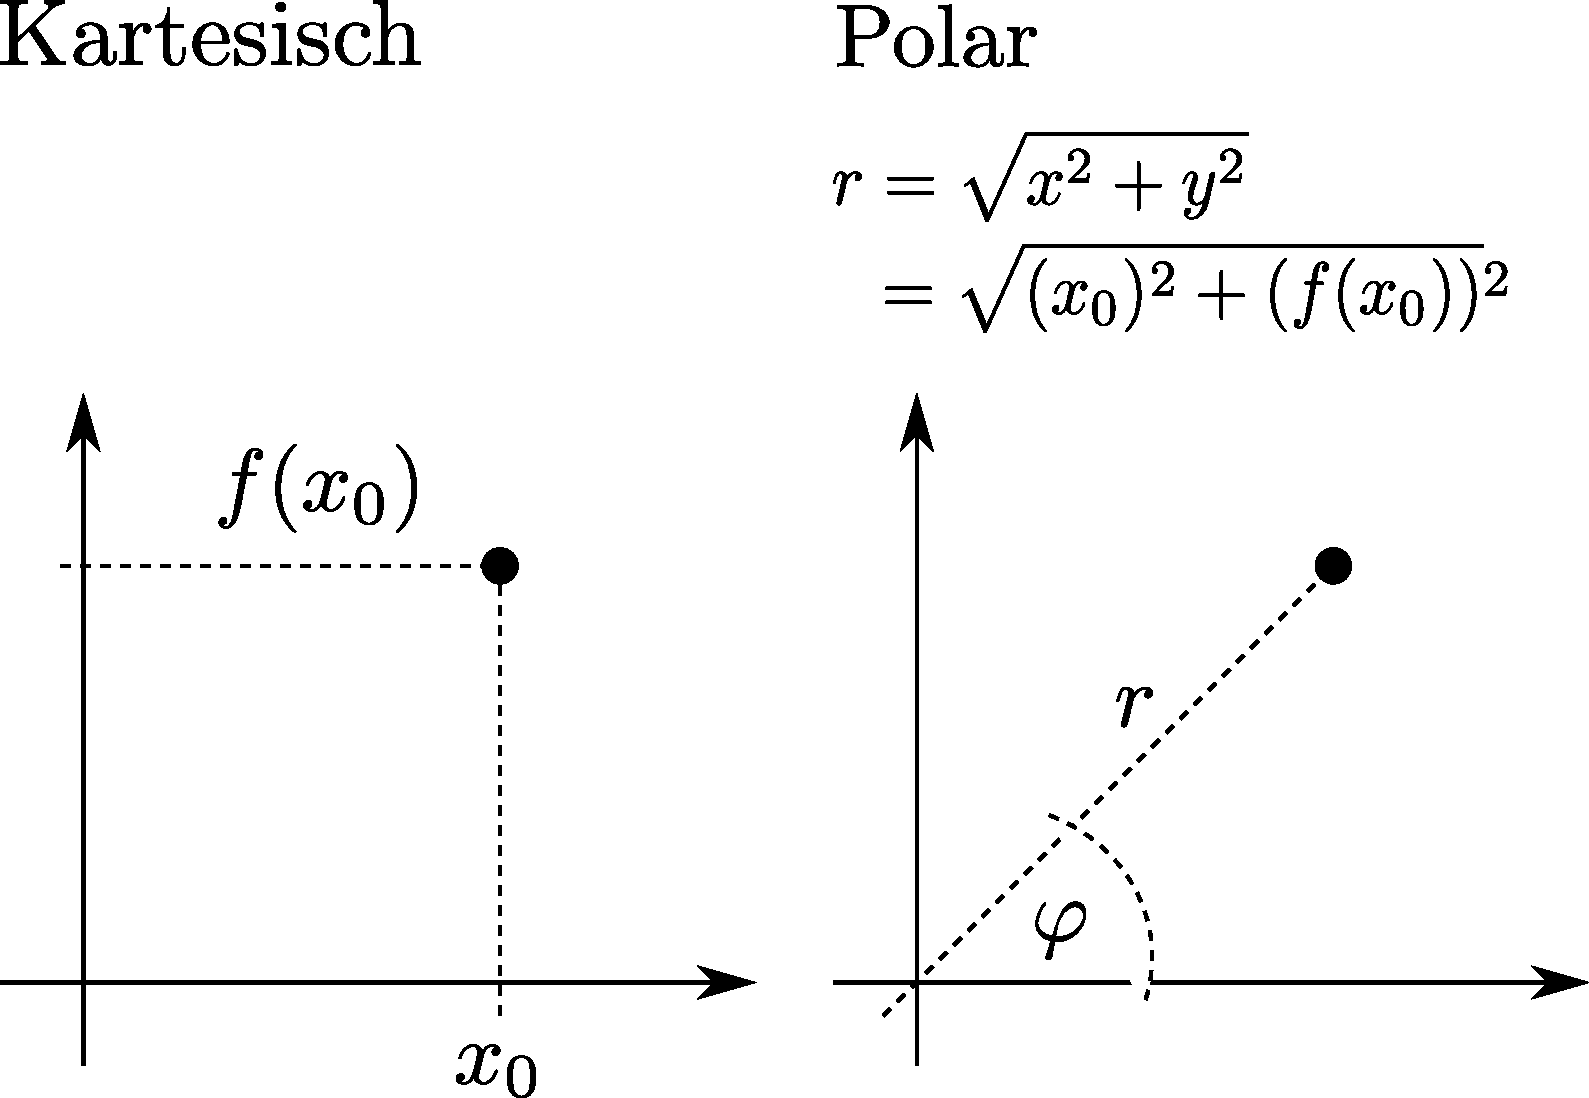
\includegraphics[width=0.6\textwidth]{../fig/polar.pdf}
\end{figure}

% \begin{figure}[h!]
%\includegraphics[height=1\textwidth,angle=270]{../fig/polar_2.pdf}
%\end{figure}

\subsection{Umrechnung Kartesisch $\rightarrow$ Polar}
\[ \boxed{r = \sqrt{x^2 + y^2}} \]
\[ \boxed{\varphi = \arctan\left(\frac{y}{x}\right)} \]
\textbf{Achtung!} Bei $\arctan()$ geht die Information über den Quadrant, in 
dem sich der Punkt befindet, verloren. Daher muss aufgrund der Vorzeichen der 
kartesischen Koordinaten entschieden werden, ob der Winkel stimmt. Ist der 
y-Achsenabschnitt positiv, so liegt $\varphi$ zwischen $0$ und $\pi$ bzw. 
$180^\circ$. Bei negativem Vorzeichen liegt $\varphi$ zwischen $-pi$ bzw. 
$-180^\circ$ und 0. 

\subsection{Umrechnung Polar $\rightarrow$ Kartesisch}
\[ \boxed{x = r \cdot \cos{\varphi}} \]
\[ \boxed{y = r \cdot \sin{\varphi}} \]

\subsection{Parameterdarstellung}
Bei der Paramaterdarstellung wird jeder Punkt durch die x- und die y-Koordinate 
definiert. 
\[ \boxed{\vec{r}(t) = \left(\begin{matrix} x(t)\\ y(t) \end{matrix}\right)} \] 

\subsubsection{Geraden}
Für die Gerade zwischen zwei Punkten $\vec{A}$ und $\vec{B}$, ausgehend von 
$\vec{A}$ nach $\vec{B}$, kann die Parameterform allgemein als 
\[ \vec{r}(t) = \overrightarrow{OA} + t \cdot \overrightarrow{AB} 
	= \begin{pmatrix} A_x \\ A_y \\ A_z \end{pmatrix} +
		t \cdot 
		\begin{pmatrix} B_x-A_x \\ B_y-A_y \\ B_z-A_z \end{pmatrix} \]
beschrieben werden.

\begin{figure}[h!]
	\centering
	\begin{tikzpicture}[domain=-1:4]
		\draw[->] (-0.5,0) -- (4,0) node[right] {$x$};
		\draw[->] (0,-0.5) -- (0, 3) node[above] {$y$};

		\draw[] (1.5,2) circle (1pt) node[above] {$A$};
		\draw[] (4,2.5) circle (1pt) node[above] {$B$};

		\draw[->, dotted] (0,0) -- (1.5,2) node[midway, sloped, above] {$\overrightarrow{OA}$};
		\draw[->, thick, red] (1.5,2) -- (4, 2.5) node[midway, sloped, above] {$\overrightarrow{AB}$};
	\end{tikzpicture}
\end{figure}

\subsubsection{Ebenen}
Analog zum Verfahren bei Geraden, kann auch für die Ebene eine 
Parameterdarstellung aufgestellt werden. Hierzu wird die Beziehung
lediglich erweitert um eine weitere Richtung, welche eine Fläche 
Aufspannt zwischen drei Punkten $A$,$B$ und $C$.

\[ \vec{r}(t) = \overrightarrow{OA} + t_1 \cdot \overrightarrow{AB} + t_2 \cdot \overrightarrow{AC} 
	= \begin{pmatrix} A_x \\ A_y \\ A_z \end{pmatrix} + t_1 
		\cdot \begin{pmatrix} B_x-A_x \\ B_y-A_y \\ B_z-A_z \end{pmatrix}
		+ t_2 \cdot \begin{pmatrix} C_x-A_x \\ C_y-A_y \\ C_z-A_z \end{pmatrix}
\]

\begin{figure}[h!]
	\centering
	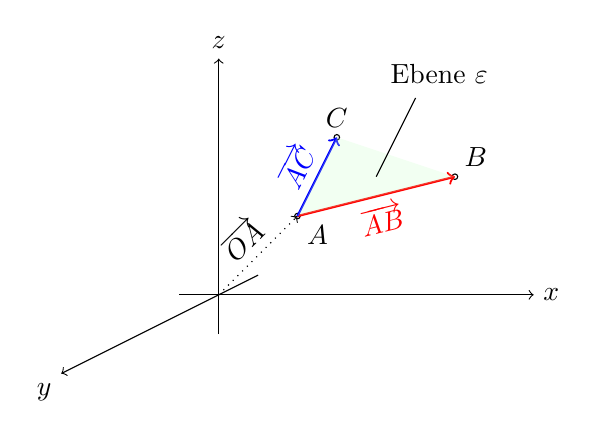
\begin{tikzpicture}[domain=-1:4]
		\draw[->] (-0.5,0) -- (4,0) node[right] {$x$};
		\draw[->] (0,-0.5) -- (0, 3) node[above] {$z$};
		\draw[->] (0.5, 0.25) -- (-2,-1) node[below left] {$y$};

		\draw[] (1,1) circle (1pt) node[below right] {$A$};
		\draw[] (3,1.5) circle (1pt) node[above right] {$B$};
		\draw[] (1.5,2) circle (1pt) node[above] {$C$};
		
		\draw[->, dotted] (0,0) -- (1,1) node[midway, sloped, above] {$\overrightarrow{OA}$};
		\draw[->, red, thick] (1,1) -- (3,1.5) node[midway, sloped, below] {$\overrightarrow{AB}$};
		\draw[->, blue, thick] (1,1) -- (1.5, 2) node[midway, sloped, above] {$\overrightarrow{AC}$};
		\fill[green!20, nearly transparent] (1,1) -- (3,1.5) -- (1.5,2) -- (1,1) -- cycle;

		\draw[] (2.8,2.8) node[] {Ebene $\varepsilon$};
		\draw[] (2.5,2.5) -- (2,1.5); 
	\end{tikzpicture}
\end{figure}

\subsubsection{Beliebige Funktionen}
Für eine beliebige Funktion im Raum erhält man die Parameterdarstellung
am einfachsten, wenn eine der Komponenten gleich $t$ gewählt wird, z.B.
$x(t)=t$. Die anderen Komponenten werden dann dieser Wahl ensprechend
angepasst. Die Funktion $y=x^2$ beispielsweise wird mit der Wahl 
$x(t) = t$ zu
\[ \vec{r}(t) = \begin{pmatrix} t \\ t^2 \end{pmatrix} \]

\begin{figure}[h!]
	\centering
	\begin{tikzpicture}[domain=-1.5:1.5]
		\draw[->] (-2.2,0) -- (2.2,0) node[right] {$x$};
		\draw[->] (0,-2.2) -- (0,2.2) node[above] {$y$};
		\draw[color=red] plot[id=x] function{x**2} node[right] {$y=x^2$};
	\end{tikzpicture}
\end{figure}

\subsubsection{Kreise}
Kreise werden generell mittels Sinus- und Kosinuskomponenten dargestellt.
Handelt es sich dabei um einen Kreis mit Mittelpunkt in $O(0|0)$ mit Radius
$r=1$ so kann dieser dargestellt werden als
\[ \vec{r}(t) = \begin{pmatrix} \cos(t) \\ \sin(t) \end{pmatrix} 
	\quad , 0 \leq t < 2\pi \]

\begin{figure}[h!]
	\centering
	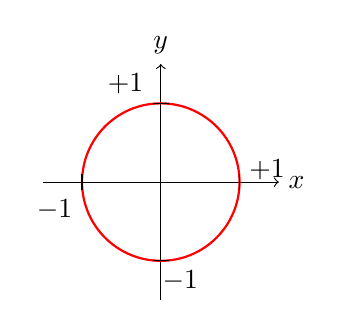
\begin{tikzpicture}[domain=-2:2]
		\draw[->] (-1.5,0) -- (1.5,0) node[right] {$x$};
		\draw[->] (0,-1.5) -- (0,1.5) node[above] {$y$};

		\draw[thick, red] (0,0) circle (1); 

		\draw[] (-1,0.1) -- (-1,-0.1) node[below left] {$-1$};
		\draw[] (1,0.1) -- (1,-0.1) node[above right] {$+1$};
		\draw[] (0.1,1) -- (-0.1,1) node[above left] {$+1$};
		\draw[] (0.1,-1) -- (-0.1,-1) node[below right] {$-1$};
	\end{tikzpicture}
\end{figure}

\subsubsection{Ellipsen}
Ein Kreis lässt sich modifizieren zu einer Ellipse mittels den 
Amplituden $A_n$ und Versätzen $b_n$ zu
\[ \vec{r}(t) = \begin{pmatrix} A_1 \cdot cos(t) + b_1 
	\\ A_2 \cdot sin(t) + b_2 \end{pmatrix} \quad ,0 \leq t < 2\pi \]

\begin{figure}[h!]
	\centering
	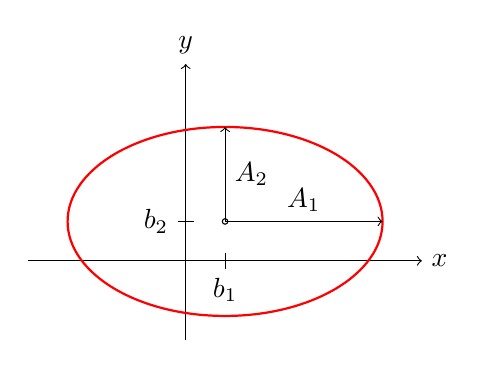
\begin{tikzpicture}[domain=-2:2]
		\draw[->] (-2,0) -- (3,0) node[right] {$x$};
		\draw[->] (0,-1) -- (0,2.5) node[above] {$y$};

		\draw[thick, red] (0.5,0.5) ellipse  (2 and 1.2); 

		\draw[] (0.5, 0.5) circle (1pt) node[below left] {};

		\draw[] (0.5,0.1) -- (0.5,-0.1) node[below] {$b_1$};
		\draw[] (0.1,0.5) -- (-0.1,0.5) node[left] {$b_2$};

		\draw[->] (0.5,0.5) -- (0.5,1.7) node[midway, right] {$A_2$};
		\draw[->] (0.5,0.5) -- (2.5,0.5) node[midway, above] {$A_1$};
	\end{tikzpicture}
\end{figure}


\subsubsection{Differential}
Die Ableitung von Funktionen in der Parameterdarstellung wird im Abschnitt
\ref{subsec:ableitungsregeln} (Seite \pageref{subsec:ableitungsregeln})
behandelt. Die partielle Ableitung, also der Gradienti, wird im Abschnitt
\ref{sec:gradient} (Seite \pageref{sec:gradient}) erläutert.
